% Color map from based on http://colorbrewer2.org/
%  * colorblind safe
%  * print friendly
%  * for sequential data
\definecolor{c1}{rgb}{0.9961, 0.9412, 0.8510}%
\definecolor{c2}{rgb}{0.9922, 0.8000, 0.5412}%
\definecolor{c3}{rgb}{0.9882, 0.5529, 0.3490}%
\definecolor{c4}{rgb}{0.8431, 0.1882, 0.1216}%

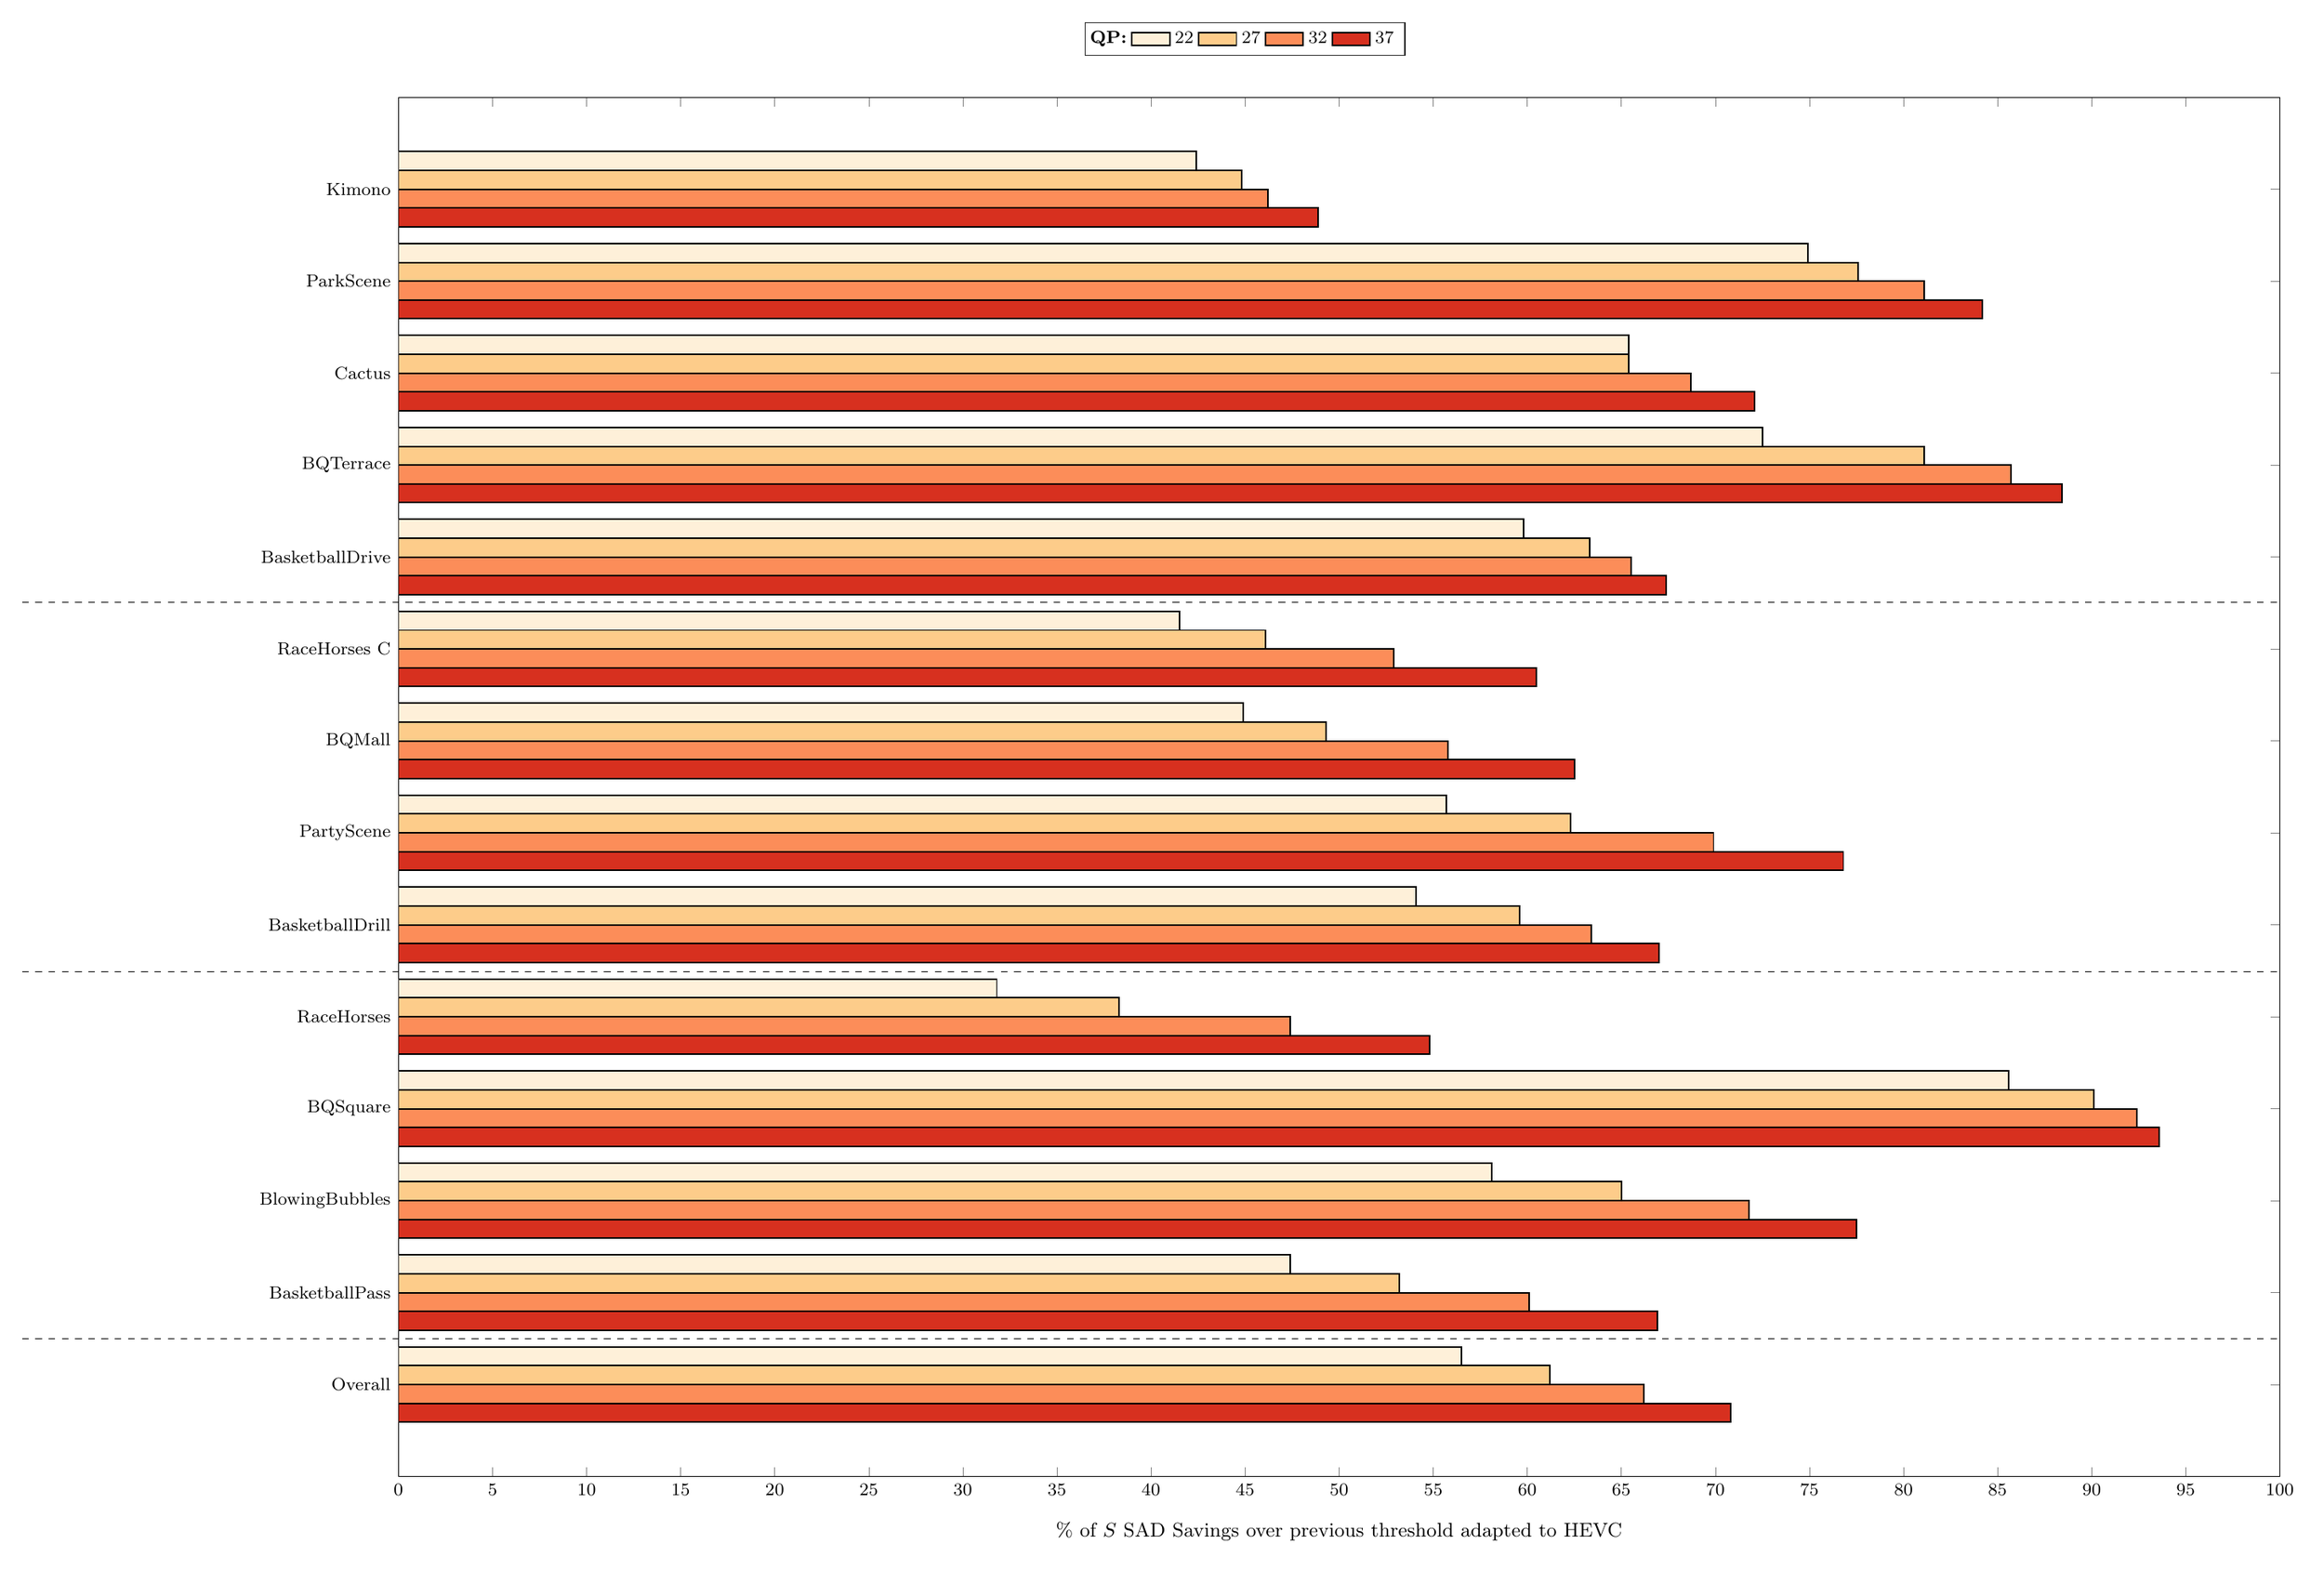
\begin{tikzpicture}

\begin{axis}[%
width=30cm,
height=22cm,
at={(0in,0in)},
scale only axis,
xmin=0,
xmax=100,
xlabel={\small{\% of $\mathbb{S}$ SAD Savings over previous threshold adapted to HEVC}},
xlabel style={yshift=-0.5em},
every x tick label/.append style={font=\color{black}\footnotesize},
ymin=0,
ymax=15,
ytick={1,2,3,4,5,6,7,8,9,10,11,12,13,14},
yticklabels={{Overall},{BasketballPass},{BlowingBubbles},{BQSquare},{RaceHorses},{BasketballDrill},{PartyScene},{BQMall},{RaceHorses C},{BasketballDrive},{BQTerrace},{Cactus},{ParkScene},{Kimono}},
axis background/.style={fill=white, font=\footnotesize},
every y tick label/.append style={font=\color{black}\footnotesize},
legend style={at={(0.45,1.03)},anchor=south,legend columns=6,legend cell align=left,align=left,draw=white!15!black,font=\footnotesize,
reverse legend}
]

\addplot[xbar,bar width=3mm,bar shift=-4.5mm,draw=black,fill=c4,line width=0.25mm,area legend] plot table[row sep=crcr] {%
70.8	1\\
66.9	2\\
77.5	3\\
93.6	4\\
54.8	5\\
67.0	6\\
76.8	7\\
62.5	8\\
60.5	9\\
67.4	10\\
88.4	11\\
72.1	12\\
84.2	13\\
48.9	14\\
};
\addlegendentry{37};

\addplot[xbar,bar width=3mm,bar shift=-1.5mm,draw=black,fill=c3,line width=0.25mm,area legend] plot table[row sep=crcr]
{%
66.2	1\\
60.1	2\\
71.8	3\\
92.4	4\\
47.4	5\\
63.4	6\\
69.9	7\\
55.8	8\\
52.9	9\\
65.5	10\\
85.7	11\\
68.7	12\\
81.1	13\\
46.2	14\\
};
\addlegendentry{32};

\addplot[xbar,bar width=3mm,bar shift=1.5mm,draw=black,fill=c2,line width=0.25mm,area legend] plot table[row sep=crcr]
{%
61.2	1\\
53.2	2\\
65	3\\
90.1	4\\
38.3	5\\
59.6	6\\
62.3	7\\
49.3	8\\
46.1	9\\
63.3	10\\
81.1	11\\
65.4	12\\
77.6	13\\
44.8	14\\
};
\addlegendentry{27};

\addplot[xbar,bar width=3mm,bar shift=4.5mm,draw=black,fill=c1,line width=0.25mm,area legend] plot table[row sep=crcr] {%
56.5	1\\
47.4	2\\
58.1	3\\
85.6	4\\
31.8	5\\
54.1	6\\
55.7	7\\
44.9	8\\
41.5	9\\
59.8	10\\
72.5	11\\
65.4	12\\
74.9	13\\
42.4	14\\
};
\addlegendentry{22};

\addlegendimage{empty legend}
\addlegendentry{\hspace{-.1cm}\textbf{QP:}}

\end{axis}
\draw[line width=0.02mm, black, dashed] (-6,2.2) -- (30,2.2);
\draw[line width=0.05mm, black, dashed] (-6,8.05) -- (30,8.05);
\draw[line width=0.05mm, black, dashed] (-6,13.95) -- (30,13.95);
\end{tikzpicture}%